\documentclass[a4paper]{IEEEtran}
\usepackage[utf8]{inputenc}
\usepackage{graphicx}
\usepackage{fontspec}   %加這個就可以設定字體
\usepackage{xeCJK}       %讓中英文字體分開設置
\usepackage{amsmath}
\usepackage{listings}
\usepackage{xcolor}
\setCJKmainfont{標楷體} %設定中文為系統上的字型,而英文不去更動,使用原TeX字型
\XeTeXlinebreaklocale "zh"             %這兩行一定要加,中文才能自動換行
\XeTeXlinebreakskip = 0pt plus 1pt     %這兩行一定要加,中文才能自動換行
\graphicspath{ {img/} }
\title{%
    Mobile Management with Hard-Handoff Criteria \\{\large Team 15, Introduction To Wireless Mobile Network ( 105-2 )}
}
\author{謝秉昂(B03901195), 謝宗宏(B02608032), 許秉鈞(B03901023)}
\begin{document}
\maketitle
\section{\textbf{ABSTRACT}}
Handover is the component that exchanges a continuous starting with one cell then onto the next as a client travels through the scope range of a cellular framework. As littler cells are deployed to meet the requests for expanded limit, the quantity of cell limit intersections increments. Every handover requires arrange assets to reroute the call to the new base station. To take care of the developing demand for very portable remote correspondence administrations, cell framework suppliers will keep on deploying extra cell destinations and present progressively complex frameworks, for both the radio connection and the system foundation. As more clients are upheld, the steadily developing concerns with respect to the restrictions of switching and signaling the infrastractures have been met by a various suite of structural and algorithmic techniques.



\section{\textbf{INTRODUCTION}}
One of the most handoff administration issues is introduced by the utilization of various path loss models. It manages the expansion of the Gaussian noise and hysteresis margin in the models to keep away from the ping-pong effect and which cell to hand over in cellular network. Our main idea is that considering different factors in handoff criteria, and use different criteria to see the results of handoff and illustrate it with plots. we've also tried to gain some insight of these simulations.
\begin{figure}[h]
    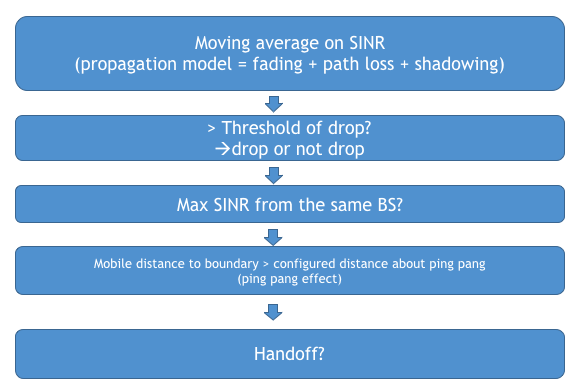
\includegraphics[width=0.45\textwidth]{diagram/1}
    \caption{Our handover machanism}
\end{figure}
If the threshold of drop become higher, the users drop timing will be bigger, and the sum of both will result in the number of handover events become fewer, which is what we expected. \\
For the possible handoff criteria, the factors are listed below:
\begin{enumerate}
\item{signal}
\item{SINR}
\item{ $\delta$ in ping pong effect}
\item{samples of observation(due to fading effect)}
\end{enumerate}
In short, We designed three criteria based on different factors and compare its performance.
\section{\textbf{RELATED WORK}}
The need to start handoff emerges when the signal of the serving base station decays underneath the threshold value. This handoff administration scheme embraces a hard handoff, which adaptively control the handoff time as indicated by the load status of cells. The displayed scheme supports better administration quality for various sort of systems utilizing different calculations. In a wireless mobile communication system, mobiles moving around the service area require communication services as a remote association. In this communication system, the coverage area is partitioned into littler locales (cells) to permit the reuse of the frequency spectrum to expand the total network capacity. The total network capacity with great quality ( and with minimum noise) is constantly attractive, frequencies utilized as a part of one cell group can be reused in different cells. Every cell is controlled by its own transmitter and receiver to serve the mobiles inside its range. The choice to start a handover relies on upon various control factors. The estimation of received signal strength must be found the averaged value of after some time to remove the quick flucthations due to the so-called multipath propagation. Averaging windows change in their shape and length, where the received signal is excessively feeble or is perilously close, making it impossible to winding up noticeably excessively weak, and then handover is required. Thus, we must ask the following questions:
\begin{itemize}
\item{Does a user get admitted?}
\item{Does a call get prematurely terminated?}
\item{How many handovers are made, and are they necessary to meet the quality of service?}
\item{How far into the coverage area of another cell does a user drift?}
\item{What is the duration of service interruption during a handover?}
\end{itemize}
A threshold level may give a trigger to start a handover, keeping a client from bouncing forward and backward between two base stations is another important issue in handover calculation outline.
\pagebreak

\section{\textbf{EXPERIMENTS}}

The mobile device moves in a fixed speed, but every random period of time, it will random to change the direction of movement. As the simulation process, mobile device movement is random, in order to reduce the single experimental error, so the same parameters are repeated using a number of experiments, the data obtained from the average.
\subsection{Handoff Threshold}
Handoff threshold is set to: when the average SINR below this value, began to prepare handoff.
\begin{enumerate}
\item{Dropout decreases as the handoff threshold rises and is expected to be the same, and the earlier handoff time is more abundant, but there may be too early problems, and the results are actually reflected in the ping pong effect, just like what we've expected.}
\item{Handoff threshold is expected to increase handoff, ping-pong will rise
(Handoff threshold infinite that mobile device will always try to connect to the SINR largest base station)}
\end{enumerate}
Initially we set the experiment only from the handoff threshold = $10^{-10}$ to $10^{-5}$ after rendering like a random distribution does not see any feature, and then from the experimental test to 1e-1 we found threshold on the ping-pong and handoff impact. There is a significant change from the beginning of the threshold = 0.001, which may mean that on the basis of this simulation setting, at the time of the order of the value = 0.001, it is the best way to distinguish between those who should not handoff This is worth the time to cause a large number of ping pong, below this value, the degree of identification is not enough, no matter what the difference is.

\begin{figure}[h]
    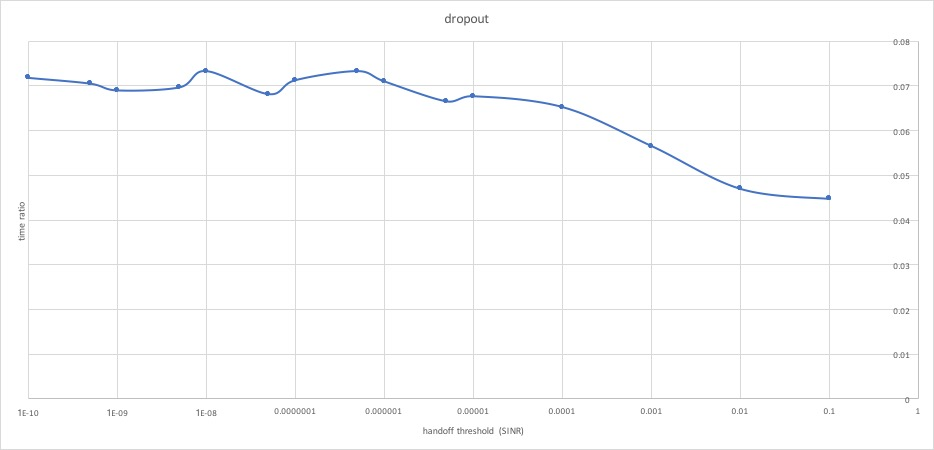
\includegraphics[width=0.45\textwidth]{handoffthreshold/dropout}
    \caption{Handoff Threshold - Dropout}
    \label{fig:mesh1}
\end{figure}
\begin{figure}[h]
    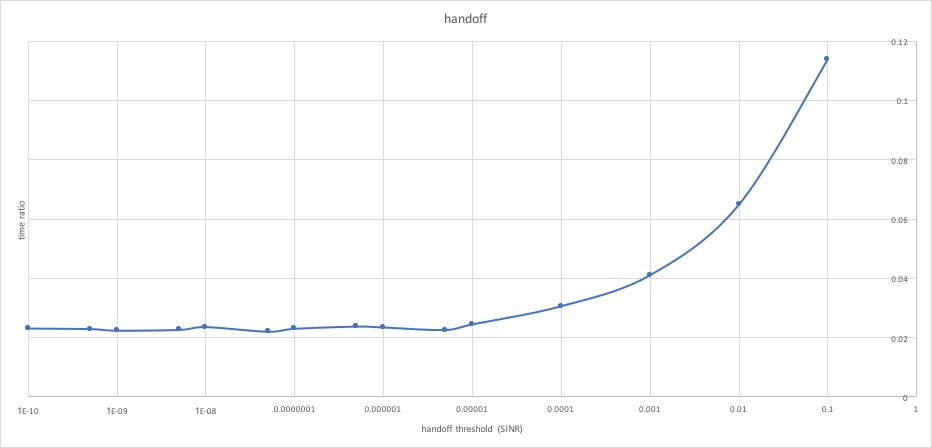
\includegraphics[width=0.35\textwidth]{handoffthreshold/handoff}
    \caption{Handoff Threshold - Handoff}
    \label{fig:mesh2}
\end{figure}
\begin{figure}[h]
    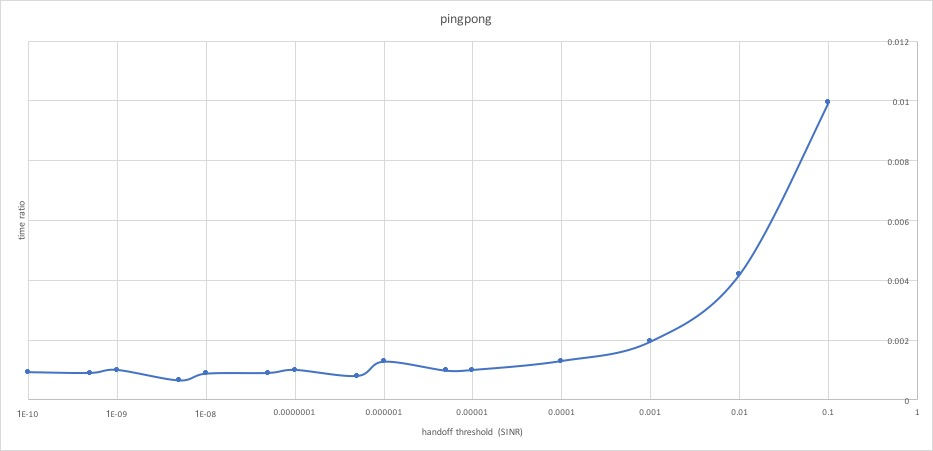
\includegraphics[width=0.45\textwidth]{handoffthreshold/pingpong}
    \caption{Handoff Threshold - Pingpong}
    \label{fig:mesh3}
\end{figure}
\subsection{Mobility}
The three values ​​increase approximately as the mobility increases, which is consistent with the expected number of nodes because the total moving path is longer and the number of base stations passed.
\begin{figure}[h]
    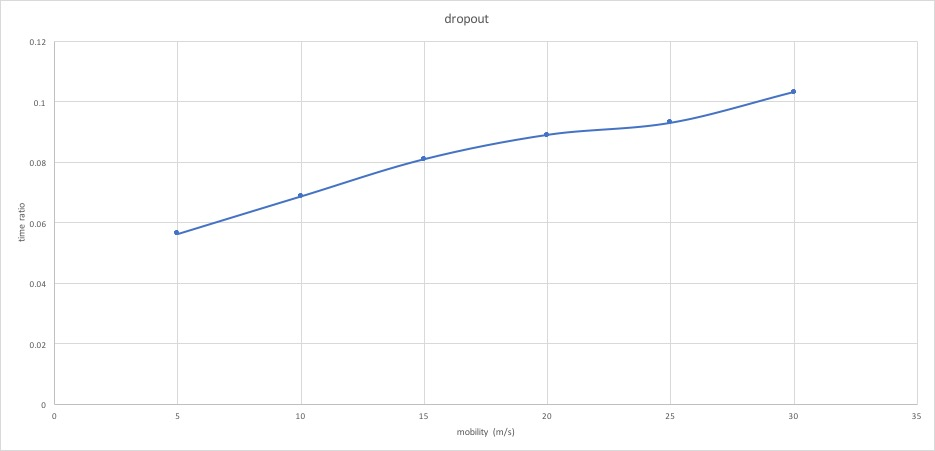
\includegraphics[width=0.45\textwidth]{mobility/dropout}
    \caption{Mobility - Dropout}
    \label{fig:mesh4}
\end{figure}
\begin{figure}[h]
    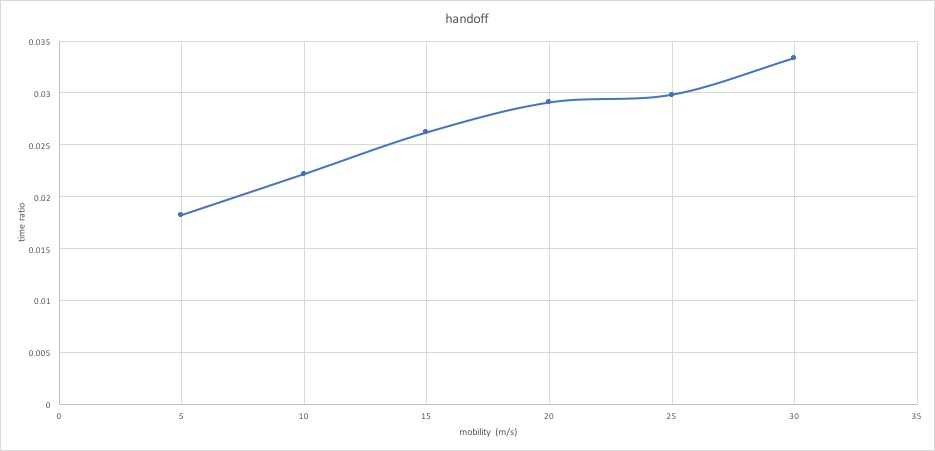
\includegraphics[width=0.45\textwidth]{mobility/handoff}
    \caption{Mobility - Handoff}
    \label{fig:mesh5}
\end{figure}
\begin{figure}[h]
    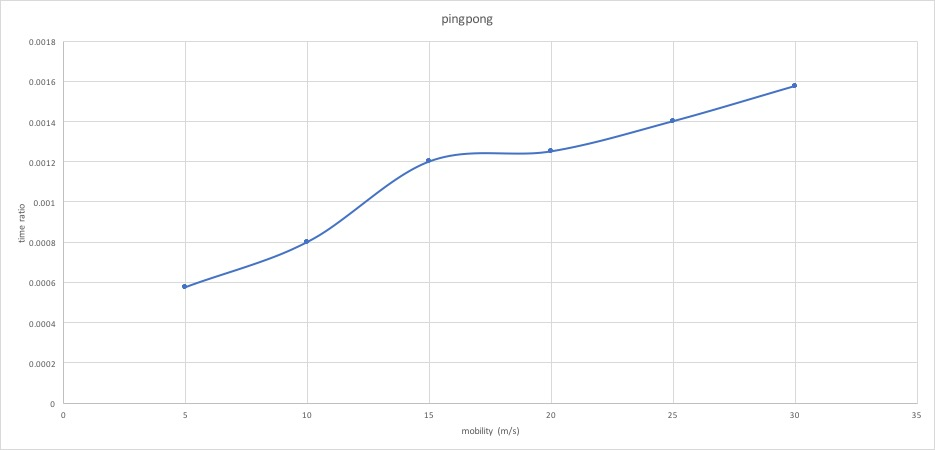
\includegraphics[width=0.45\textwidth]{mobility/pingpong}
    \caption{Mobility - Pingpong}
    \label{fig:mesh6}
\end{figure}
\subsection{Take A Closer Look}
If we take those data described above into account, says, those three values ​​of which increase approximately as the mobility increases, which is consistent with the expected number of nodes because the total moving path is longer and the number of base stations passed. We can get the following results.
\begin{figure}[h]
    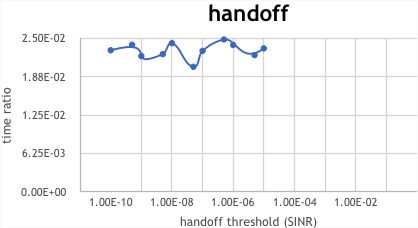
\includegraphics[width=0.45\textwidth]{small/dropout}
    \caption{Mobility - Dropout}
    \label{fig:mesh7}
\end{figure}
\begin{figure}[h]
        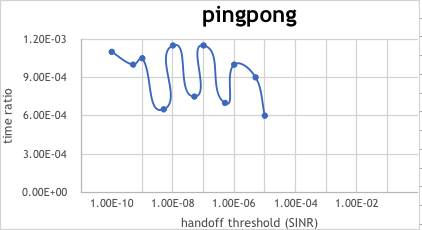
\includegraphics[width=0.45\textwidth]{small/handoff}
    \caption{Mobility - Handoff}
    \label{fig:mesh8}
\end{figure}
\begin{figure}[h]
    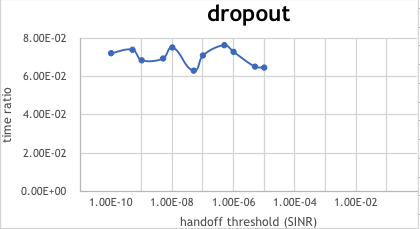
\includegraphics[width=0.45\textwidth]{small/pingpong}
    \caption{Mobility - Pingpong}
    \label{fig:mesh9}
\end{figure}
\section{\textbf{CONCLUSION}}
A gathering of clients with a huge scope of versatility can access around in the general system creating substantial stream of traffic. At the point when the movement stack is concentrated in a cell, this cell turns into the so-called hotspot cell [1]. Thus, there is a need an appropriate activity driven handoff criteria; with the goal that clients will naturally move from congested cell to enable the system to adjust itself progressively.

\section{\textbf{REFERENCES}}

[1] Michel Goossens, Frank Mittelbach, and Alexander Samarin.
\textit{The \LaTeX\ Companion}.
Addison-Wesley, Reading, Massachusetts, 1993.

[2] Albert Einstein.
\textit{Zur Elektrodynamik bewegter K{\"o}rper}. (German)
[\textit{On the electrodynamics of moving bodies}].
Annalen der Physik, 322(10):891–921, 1905.


[3] Knuth: Computers and Typesetting,
\\\texttt{http://www-cs-faculty.stanford.edu/\~{}uno/abcde.html}

\end{document}
